\documentclass{standalone}
\usepackage{tikz}
\usetikzlibrary{arrows,calc}

\begin{document}

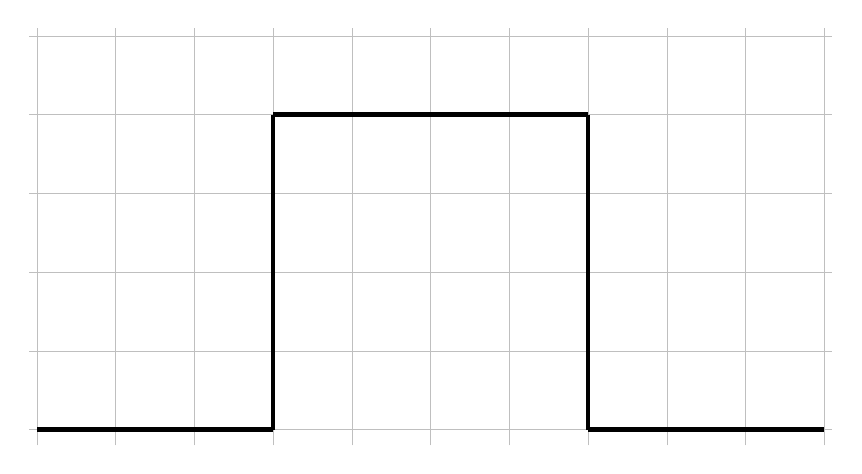
\begin{tikzpicture}
    \draw[very thin,color=gray!50] (-5.1,-0.2) grid (5.1,5.1);
%    \draw[->] (-5.2,0) -- (5.2,0) node[right] {$x$};
%    \draw[->] (0,-0.2) -- (0,5.2) node[above] {$f(x)$};
    \draw[-,ultra thick] (-2,4) -- (2,4) node[above] {};
    \draw[-,ultra thick] (-2,0) -- (-2,4) node[above] {};
    \draw[-,ultra thick] (2,0) -- (2,4) node[above] {};
    \draw[-,ultra thick] (2,0) -- (5,0) node[above] {};
    \draw[-,ultra thick] (-2,0) -- (-5,0) node[above] {};
\end{tikzpicture}
\end{document} 
